\documentclass[12pt]{beamer}
\usetheme{default}
\usecolortheme{beetle}

\usepackage[utf8]{inputenc}
\usepackage[english]{babel}
\usepackage{amsmath}
\usepackage{amsfonts}
\usepackage{amssymb}
\usepackage{graphicx}
\usepackage{tikz}
\usetikzlibrary{positioning}
\usepackage{listings}
\usepackage{xcolor}
\usepackage{fontawesome}
\usepackage{marvosym}
\usepackage{romannum}

\title{Graph Data - Modelling and Querying}
\subtitle{with Neo4j and Cypher}
\author[I.Feuerstein]{Iryna Feuerstein}
\institute[Meetup]{Graph Database - NRW Meetup}
\titlegraphic{
\includegraphics[height=0.6cm]{pd_logo.png}}
%\logo{
\includegraphics[height=0.7cm]{logo.png}\vspace{230pt}}
\date{6 December 2017}
\setbeamertemplate{background}
{
\includegraphics[width=\paperwidth,height=\paperheight,keepaspectratio]{background.png}}
\begin{document}
    
    \begin{frame}
        \frametitle{Introduction}
        Please find two other learning partners, 
        \begin{itemize}
            \item form a standing group and 
            \item tell them what you already know about \begin{itemize}
                \item graphs, 
                \item graph databases and 
                \item Neo4j.
            \end{itemize}
        \end{itemize}
    \end{frame}
    
    \maketitle
    
    \begin{frame}
        \frametitle{Learning goals}
        \tableofcontents
    \end{frame}
    
    \section{What are graphs?}
    \subsection{Definition}
    
    \begin{frame}
        \frametitle{Graph}
        \begin{Definition}
            \emph{Graph} is an ordered pair \(G = \left(V,E\right)\) comprising a set \(V\) of \emph{vertices}, \emph{nodes} or \emph{points} together with a set \(E\) of \emph{edges}, \emph{arcs} or \emph{lines}, which are 2-element subsets of V.\footnotemark
        \end{Definition}
        \pause
        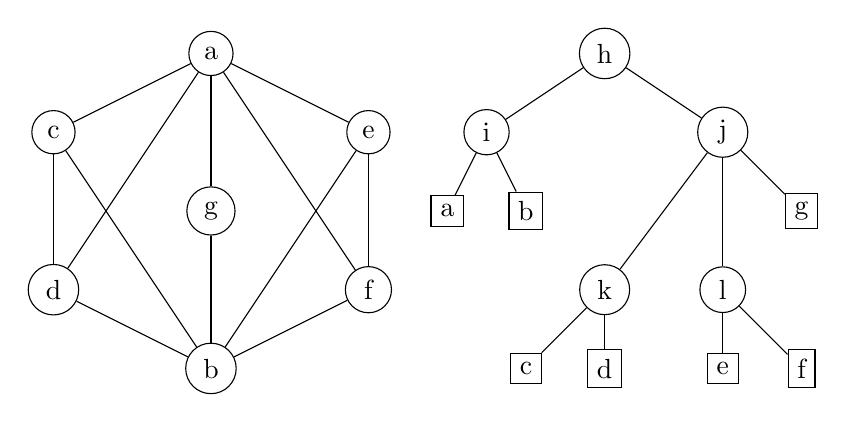
\begin{tikzpicture}
        \node[draw, circle] (a) at (3,4){a};
        \node[draw, circle] (b) at (3,0){b};
        \node[draw, circle] (c) at (1,3){c};
        \node[draw, circle] (d) at (1,1){d};
        \node[draw, circle] (e) at (5,3){e};
        \node[draw, circle] (f) at (5,1){f};
        \node[draw, circle] (g) at (3,2){g};
        \draw[-] (a)--(c);
        \draw[-] (a)--(d);
        \draw[-] (a)--(e);
        \draw[-] (a)--(f);
        \draw[-] (a)--(g);
        \draw[-] (b)--(c);
        \draw[-] (b)--(d);
        \draw[-] (b)--(e);
        \draw[-] (b)--(f);
        \draw[-] (b)--(g);
        \draw[-] (c)--(d);
        \draw[-] (e)--(f);
        
        \node[draw, circle](root) at (8,4){h};
        \node[draw, circle](ab) at (6.5,3){i};
        \node[draw, circle](root-g) at (9.5,3){j};
        \node[draw, circle](cd) at (8,1){k};
        \node[draw, circle](ef) at (9.5,1){l};
        \node[draw](a) at (6,2) {a};
        \node[draw](b) at (7,2) {b};
        \node[draw](c) at (7,0) {c};
        \node[draw](d) at (8,0) {d};
        \node[draw](e) at (9.5,0) {e};
        \node[draw](f) at (10.5,0) {f};
        \node[draw](g) at (10.5,2) {g};
        \draw [-] (root)--(ab);
        \draw [-] (root)--(root-g);
        \draw [-] (ab)--(a);
        \draw [-] (ab)--(b);
        \draw [-] (root-g)--(cd);
        \draw [-] (root-g)--(ef);
        \draw [-] (root-g)--(g);
        \draw [-] (cd)--(c);
        \draw [-] (cd)--(d);
        \draw [-] (ef)--(e);
        \draw [-] (ef)--(f);
        \end{tikzpicture}
        \footnotetext{\url{en.wikipedia.org/wiki/Graph_(discrete_mathematics)}}
    \end{frame}
    
    \subsection{Use cases}
    \begin{frame}
        \frametitle{Use Cases}
        \begin{itemize}
            \pause
            \item Networks
            \pause
            \begin{itemize}
                \item Social networks\\[3mm]
                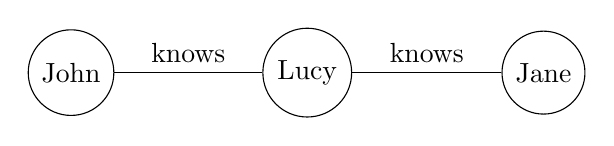
\begin{tikzpicture}
                \node[draw, circle](john) at (0,0){John};
                \node[draw, circle](lucy) at (3,0){Lucy};
                \node[draw, circle](jane) at (6,0){Jane};
                \path (john) edge node [above] {knows} (lucy);
                \path (lucy) edge node [above] {knows} (jane);
                \end{tikzpicture}
                \pause
                \item Computer networks\\[3mm]
                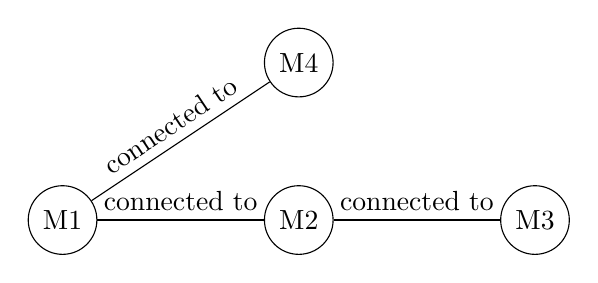
\begin{tikzpicture}
                \node[draw, circle](m1) at (0,0){M1};
                \node[draw, circle](m2) at (3,0){M2};
                \node[draw, circle](m3) at (6,0){M3};
                \node[draw, circle](m4) at (3,2){M4};
                \path (m1) edge node [above] {connected to} (m2);
                \path (m2) edge node [above] {connected to} (m3);
                \path (m1) edge node [pos=0.5, sloped, above] {connected to} (m4);
                
                \end{tikzpicture}
            \end{itemize}
        \end{itemize}
    \end{frame}
    
    \begin{frame}
        \frametitle{Use Cases}
        \begin{itemize}
            \item Networks
            \begin{itemize}
                \item Transport networks\\[3mm]
                
                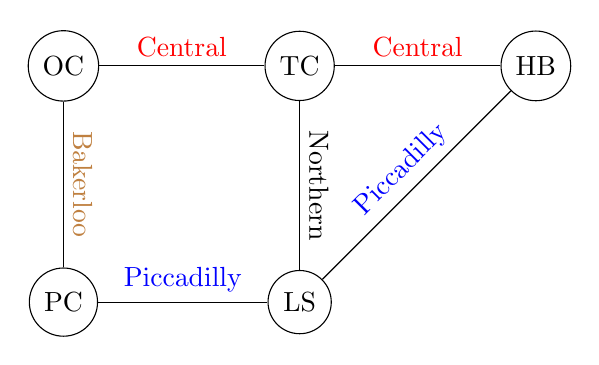
\begin{tikzpicture}
                \node[draw, circle](m1) at (0,3){OC};
                \node[draw, circle](m2) at (3,3){TC};
                \node[draw, circle](m3) at (6,3){HB};
                \node[draw, circle](m4) at (3,0){LS};
                \node[draw, circle](m5) at (0,0){PC};
                \path (m1) edge node [above, red] {Central} (m2);
                \path (m2) edge node [above, red] {Central} (m3);
                \path (m3) edge node [pos=0.5, sloped, above, blue] {Piccadilly} (m4);
                \path (m4) edge node [pos=0.5, sloped, above, blue] {Piccadilly} (m5);
                \path (m1) edge node [pos=0.5, sloped, above, brown] {Bakerloo} (m5);
                \path (m2) edge node [pos=0.5, sloped, above] {Northern} (m4);
                \end{tikzpicture}
                
            \end{itemize}
            
        \end{itemize}
        \begin{align*}
        OC & = & \text{Oxford Circus} &,& LS & = & \text{Leicester Square} \\
        HB & = & \text{Holborn} &,& PC & = & \text{Piccadilly Circus}\\
        TC & = & \text{Tottenham Court Road}\\
        \end{align*}
    \end{frame}
    
    \begin{frame}
        \frametitle{Use Cases}
        \begin{itemize}
            \item Natural Language Processing\\[3mm]
            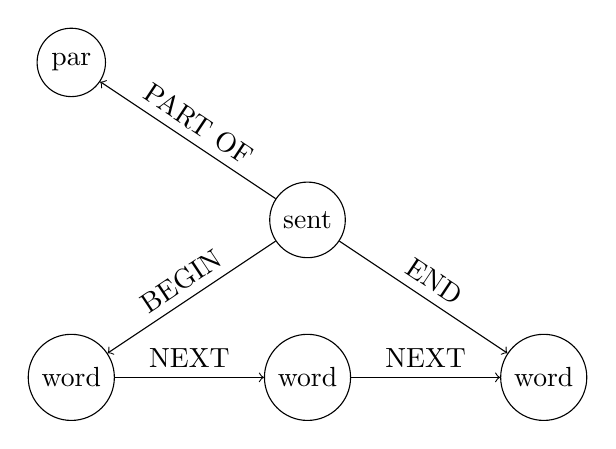
\begin{tikzpicture}
            \node[draw, circle](w1) at (0,0){word};
            \node[draw, circle](w2) at (3,0){word};
            \node[draw, circle](w3) at (6,0){word};
            \node[draw, circle](s) at (3,2){sent};
            \node[draw, circle](p) at (0,4){par};
            \path (w1) edge[->] node [above] {NEXT} (w2);
            \path (w2) edge[->] node [above] {NEXT} (w3);
            \path (s) edge[->] node [sloped, above] {BEGIN} (w1);
            \path (s) edge[->] node [sloped, above] {END} (w3);
            \path (s) edge[->] node [sloped, above] {PART OF} (p);
            \end{tikzpicture}
        \end{itemize}
    \end{frame}
    
    \begin{frame}
        \frametitle{Use Cases}
        \begin{itemize}
            \item Document management\\[2mm]
            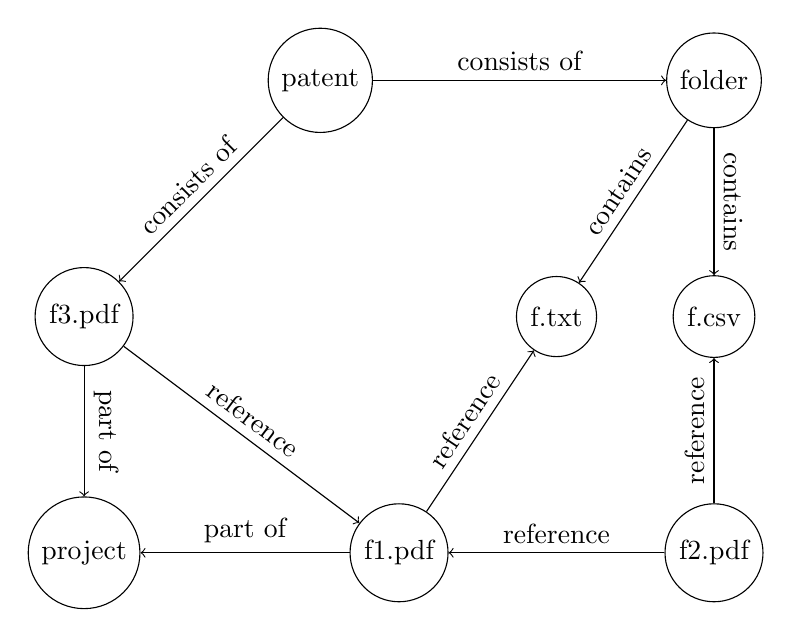
\begin{tikzpicture}
            \node[draw, circle](pr) at (0,0){project};
            \node[draw, circle](f1) at (4,0){f1.pdf};
            \node[draw, circle](f2) at (8,0){f2.pdf};
            \node[draw, circle](f3) at (0,3){f3.pdf};
            \node[draw, circle](txt) at (6,3){f.txt};
            \node[draw, circle](csv) at (8,3){f.csv};
            \node[draw, circle](pt) at (3,6){patent};
            \node[draw, circle](f) at (8,6){folder};
            \path (f1) edge[->] node [above] {part of} (pr);
            \path (f2) edge[->] node [above] {reference} (f1);
            \path (f3) edge[->] node [sloped, above] {part of} (pr);
            \path (f3) edge[->] node [sloped, above] {reference} (f1);
            \path (f1) edge[->] node [sloped, above] {reference} (txt);
            \path (f2) edge[->] node [sloped, above] {reference} (csv);
            \path (pt) edge[->] node [sloped, above] {consists of} (f3);
            \path (pt) edge[->] node [sloped, above] {consists of} (f);
            \path (f) edge[->] node [sloped, above] {contains} (txt);
            \path (f) edge[->] node [sloped, above] {contains} (csv);
            \end{tikzpicture}
        \end{itemize}
    \end{frame}
    
    \begin{frame}
        \frametitle{Use Cases}
        \begin{itemize}
            \item Biochemistry / Genomics\\[2mm]
            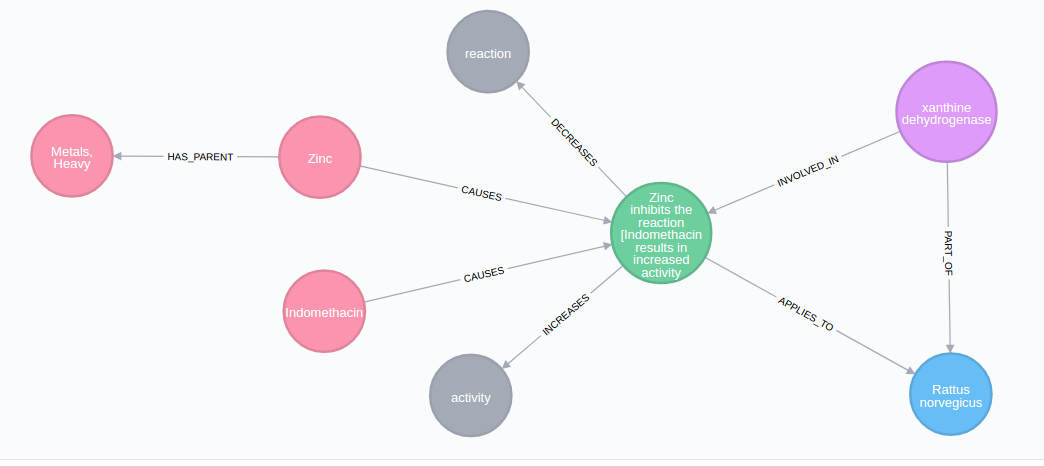
\includegraphics[width=0.9\textwidth]{genomics.png}
        \end{itemize}
        \footnotetext{\url{http://ctdbase.org/}}
    \end{frame}
    
    \begin{frame}{Practice activity - Graph modeling}
        \begin{itemize}
            \item Come up with any use case idea of your choice. 
            \item Model it as a graph on a sheet of paper. 
            \item Introduce it to at least one of the attendees.
        \end{itemize}
    \end{frame}
        
    \section{Starting with Neo4j and Cypher}
    \subsection{Configuration and start}
    \begin{frame}
        \frametitle{Installation}
        \begin{itemize}
            \item Find the right installation file for your OS at \textcolor{white}{\url{neo4j-training-files/neo4j}} on the flash drive and install the software.
            \pause
            \item Linux-Users: Copy both JAR-files from the \textcolor{white}{\url{neo4j-training-files/plugins}} directory into \textcolor{white}{\url{NEO4J_HOME/plugins}} directory of your Neo4j installation.
            \pause
            \item Mac-Users: Copy the plugins directory into your \textcolor{white}{\url{/Application/Neo...}} and into \textcolor{white}{\url{graph.db/plugins}}
            \pause
            \item Windows-Users: Follow the installation and start client.
        \end{itemize}
    \end{frame}
    
    \begin{frame}
        \frametitle{Installation}
        \begin{itemize}
            \item Replace the \textcolor{white}{\url{NEO4J_HOME/conf/neo4j.conf}} configuration file with the one found on the flash drive at \textcolor{white}{\url{neo4j-training-files/conf/neo4j.conf}}.
            \pause
            \item Copy the \textcolor{white}{\url{neo4j-training-files/data/ctdbase.db}} folder into your \textcolor{white}{\url{NEO4J_HOME/data/databases/}} directory
        \end{itemize}
    \end{frame}
    
    \begin{frame}
        \frametitle{Starting Neo4j}
        \begin{itemize}
            \item Start the database with\\
            \textcolor{white}{\url{NEO4J_HOME/bin/neo4j} \url{console}}
            \pause
            \item Go to \textcolor{white}{\url{http://localhost:7474}} within you browser
        \end{itemize}
    \end{frame}
    
    \begin{frame}{Practice activity}
        \begin{itemize}
            \item Please separate in 4 groups:
            \begin{itemize}
                \item Chemical
                \item Disease
                \item Organism
                \item Gene
            \end{itemize}
            \pause
            \item Explore the dashboard in groups
            \item What can you find out about your node type?
            \item What questions arise?
        \end{itemize}
        
    \end{frame}
    
    \begin{frame}
        \frametitle{Demonstration}
        \begin{block}{Important configuration entries}
            dbms.active\_database=ctdbase.db\\
            dbms.security.auth\_enabled=false\\
            dbms.security.procedures.unrestricted=algo.*,apoc.*\\
            apoc.import.file.enabled=true
        \end{block}
    \end{frame}
    
    \subsection{CRUD operations with Cypher}
    \begin{frame}
        \frametitle{Live coding session - CRUD operations}
        \begin{block}{create node}
            CREATE (c:Chemical \{name: 'Helium'\})\\ 
            \hspace{1cm} RETURN c
        \end{block}
        \begin{block}{update node}
            MERGE (c:Chemical \{name: 'Helium'\})\\
            \hspace{1cm} SET c.symbol = 'He' 
            \hspace{1cm} RETURN c
        \end{block}
    \end{frame}
    
    \begin{frame}
        \frametitle{Live coding session - CRUD operations}
        \begin{block}{delete node without relations}
            MATCH (c:Chemical \{name:'Helium'\})\\
            \hspace{1cm} DELETE c
        \end{block}
        \begin{block}{delete node without relations}
            MATCH (c:Chemical)\\
            \hspace{1cm} WHERE c.name = 'Helium'\\
            \hspace{1cm} DELETE c
        \end{block}
        \begin{block}{delete node with existing relations}
            MATCH (c:Chemical \{name:'Helium'\})\\
            \hspace{1cm} DETACH DELETE c\\
        \end{block}
    \end{frame}
    
    \begin{frame}
        \frametitle{Live coding session - CRUD operations}
        \begin{block}{create relation between new nodes}
            CREATE (c:Chemical \{chemicalName:'Helium'\})\\
            \hspace{1cm} -[:BELONGS\_TO]-\textgreater\\
            \hspace{1cm} (g:ChemicalGroup \{groupName:'Noble gases'\})\\ 
            RETURN c,g
        \end{block}
        \begin{block}{create relation between existing nodes}
            MATCH (g:ChemicalGroup \{groupName:'Noble gases'\}),\\
            \hspace{1.4cm} (p:ChemicalGroup \{groupName:'Gases'\})\\
            CREATE (g)-[:HAS\_PARENT]-\textgreater(p)\\ 
            RETURN g,p
        \end{block}
    \end{frame}
    
    \begin{frame}
        \frametitle{Live coding session - CRUD operations}
        \begin{block}{update relation}
            MATCH ()-[r:BELONGS\_TO]-()\\
            \hspace{1cm} SET r.updateTime = timestamp()\\
            \hspace{1cm} RETURN r
        \end{block}
        \begin{block}{delete relation}
            MATCH ()-[r:BELONGS\_TO]-()\\
            \hspace{1cm} DELETE r
        \end{block}
    \end{frame}
    
    \begin{frame}{Practice activity}
        \begin{itemize}
            \item Go back to your graph model from the beginning of the training.
            \item Create about
            \begin{itemize}
                \item 10 nodes and
                \item 15 relations
                \item with properties.
            \end{itemize}
        \end{itemize}
    \end{frame}
    
    \frame{FINISH: PART ONE}
    
    \section{Quering for paths and patterns}
    \begin{frame}
        \frametitle{Live coding session}
        \begin{block}{Check your indexes}
            CALL db.indexes\\
            CREATE INDEX ON :Disease(diseaseId)\\
            CREATE INDEX ON :Gene(geneName, geneSymbol)\\
        \end{block}
    \end{frame}
    
    \begin{frame}{Live coding session}
        \begin{block}{Example}
            MATCH (g:Gene)\\ 
            \hspace{1cm} WHERE g.geneSymbol = 'CTSD'\\
            \hspace{1cm} RETURN g
        \end{block}
        \begin{block}{Example}
            MATCH (g:Gene)\textless-[:ASSOCIATED\_WITH]-(d:Disease)\\
            \hspace{1cm} WHERE g.geneSymbol = 'CTSD'\\
            \hspace{1cm} RETURN g, d\\
        \end{block}
        \begin{block}{Example}
            MATCH (g:Gene)\textless-[:ASSOCIATED\_WITH]-(d:Disease)\\
            \hspace{1cm} WHERE g.geneSymbol = 'CTSD'\\
            \hspace{1cm} RETURN g, count(d)\\
        \end{block}
    \end{frame}
    
    \begin{frame}{Live coding session}
        \begin{block}{Example}
            MATCH (g:Gene)\textless-[:ASSOCIATED\_WITH]-(d:Disease)\\
            \hspace{1cm} WITH g, count(d) as diseases\\
            \hspace{1cm} WHERE diseases \textgreater 50\\
            \hspace{1cm} RETURN g.geneName, g.geneSymbol, diseases\\
            \hspace{1cm} ORDER BY diseases DESC
        \end{block}
        \begin{block}{Example}
            MATCH (g:Gene)\textless-[:ASSOCIATED\_WITH]-(d:Disease)\\
            \hspace{1cm}-[:ASSOCIATED\_WITH]-\textgreater(otherGene:Gene)\\
            \hspace{1cm} WHERE g.geneSymbol = 'CTSD'\\
            RETURN otherGene.geneName, otherGene.geneSymbol
        \end{block}
    \end{frame}
    
    \begin{frame}
        \frametitle{Live coding session}
        \begin{block}{Example}
            MATCH p = (c:Chemical)-[*2]-(d:Disease)\\
            \hspace{1cm} WHERE d.diseaseName STARTS WITH 'Osteo'\\
            \hspace{1cm} RETURN p LIMIT 20
        \end{block}
        \begin{block}{Example}
            MATCH (c:Chemical)\textless-[:HAS\_PARENT*3..4]-(d:Chemical)\\ 
            \hspace{1cm} WITH c, count(d) AS descendants,\\
            \hspace{1cm} collect(d.chemicalName) AS names\\
            \hspace{1cm} ORDER BY descendants DESC LIMIT 10\\
            RETURN c.chemicalName, names[1..10], descendants
        \end{block}
    \end{frame}
    
    \begin{frame}
        \frametitle{Live coding session}
        \begin{block}{Example}
            MATCH p = (c:Chemical {chemicalName: 'Zinc Acetate'})\\
            -[:ASSOCIATED\_WITH\(|\):CAUSES\(|\):INVOLVED\_IN*1..3]-\\
            (d:Disease {diseaseName: 'Alzheimer Disease'})\\
            \hspace{1cm} RETURN p LIMIT 10
        \end{block}
        \begin{block}{Example}
            MATCH (:InteractionType \{typeName:'degradation'\})\\
            \hspace{1cm} \textless-[:INCREASES\(|\):DECREASES]-\\
            \hspace{1cm} (i:Interaction)-[:APPLIES\_TO]-\textgreater\\
            \hspace{1cm} (:Organism \{organismName:'Cricetulus griseus'\})\\
            RETURN i.description
        \end{block}
    \end{frame}

    \begin{frame}{Practice activity}
        For each group (Chemical, Disease, Organism, Gene):
        \begin{itemize}
            \item Please check your questions from the first practice activity.
            \begin{itemize}
                \item Can you answer any of them now?
            \end{itemize}
            \item Think about new questions as you explore the graph with the querying techniques just learned.
            \item Present one question, appropriate query and an answer to your classmates.
        \end{itemize}
    \end{frame}
    
    \begin{frame}{Live coding session}
        \begin{block}{Shortest path example}
            MATCH (zinc:Chemical \{chemicalName:'Zinc Acetate'\}),\\
            \hspace{1cm} (metals:Chemical \{chemicalName:'Carboxylic Acids'\}),\\
            \hspace{1cm} p = shortestPath((zinc)-[*..15]-(metals))\\
            RETURN p\\
        \end{block}
        \begin{block}{Shortest path example}
            MATCH (zinc:Chemical \{chemicalName:'Zinc Acetate'\}),\\
            \hspace{1cm} (metals:Chemical \{chemicalName:'Carboxylic Acids'\}),\\
            \hspace{1cm} p = shortestPath((zinc)-[*..15]-(metals))\\
            WHERE NONE(r IN relationships(p)\\
            \hspace{2.7cm} WHERE type(r)='CAUSES')\\
            RETURN p\\
        \end{block}
    \end{frame}
    
    \begin{frame}{Live coding session}
        \begin{block}{Shortest path example}
            MATCH (c:Chemical \{chemicalName:'Zinc Acetate'\}),\\
            \hspace{1cm} (d:Disease \{diseaseName:'Alzheimer Disease'\})\\
            MATCH path = allShortestPaths( (c)-[*..3]-(d) )\\
            RETURN path
        \end{block}
    \end{frame}
    
    \frame{FINISH: PART TWO}
    
    \section{Using graph algorithms}
    \begin{frame}
        \frametitle{Calling procedures}
        \begin{itemize}
            \item CALL db.schema
            \item CALL dbms.procedures
            \item CALL dbms.functions
            \item CALL apoc.help('dijkstra')
        \end{itemize}
    \end{frame}
    
    \subsection{apoc library}
    \begin{frame}
        \frametitle{Live coding session}
        \begin{Definition}
            In a connected graph, the normalized \emph{closeness centrality} of a node is the average length of the shortest path between the node and all other nodes in the graph. Thus the more central a node is, the closer it is to all other nodes.\footnotemark
        \end{Definition}
        \begin{block}{Closeness Centrality Example}
            MATCH (node:Chemical)\\
            \hspace{1cm} WHERE node.chemicalName CONTAINS 'Vitamin'\\
            \hspace{1cm} WITH collect(node) AS nodes\\
            CALL apoc.algo.closeness(['HAS\_PARENT'],nodes,'BOTH')\\
            \hspace{1cm} YIELD node, score\\
            RETURN node, score\\
            \hspace{1cm} ORDER BY score DESC
        \end{block}
        \footnotetext{\url{en.wikipedia.org/wiki/Centrality\#Closeness_centrality}}
    \end{frame}
    
    \begin{frame}
        \frametitle{Live coding session}
        \begin{Definition}
            \emph{Betweenness centrality} quantifies the number of times a node acts as a bridge along the shortest path between two other nodes.\footnotemark
        \end{Definition}
        \begin{block}{Betweenness Centrality Example}
            MATCH (node:Disease)\\
            \hspace{1cm} WHERE node.diseaseName CONTAINS 'deficiency'\\
            \hspace{1cm} WITH collect(node) AS nodes\\
            CALL apoc.algo.betweenness(['HAS\_PARENT'],\\
            \hspace{6cm} nodes,'BOTH')\\
            \hspace{1cm} YIELD node, score\\
            RETURN node.diseaseName, score\\
            \hspace{1cm} ORDER BY score DESC LIMIT 10
        \end{block}
        \footnotetext{\url{en.wikipedia.org/wiki/Centrality\#Betweenness_centrality}}
    \end{frame}
    
    \begin{frame}
        \frametitle{Live coding session}
        \begin{Definition}
            In graph theory, a \emph{clique} is a subset of vertices of an undirected graph such that every two distinct vertices in the clique are adjacent.
        \end{Definition}
        \begin{block}{Clique example query}
        MATCH (startNode:Category\\
        \hspace{3cm} \{name:'Endocrine system disease'\})\\
        \hspace{1cm} CALL apoc.algo.cliquesWithNode(startNode, 4)\\
        \hspace{1cm} YIELD clique\\
        RETURN clique
        \end{block}
        \footnotetext{\url{en.wikipedia.org/wiki/Clique_(graph_theory)}}
    \end{frame}
    
    \begin{frame}{Practice activity}
        Explore the APOC library:
        \begin{itemize}
            \item read the documentation,
            \item try out different queries,
            \item make notes to about your questions and results.
        \end{itemize}
    \end{frame}
    
    \subsection{algo library}
    \begin{frame}
        \frametitle{Live coding session}
        \begin{block}{PageRank example}
            CALL algo.pageRank.stream('InteractionType',\\
            \hspace{1cm} 'HAS\_PARENT', \{iterations:20\})\\
            \hspace{1cm} YIELD node, score\\
            WITH * ORDER BY score DESC LIMIT 5\\
            RETURN node.typeName, node.code, score;
        \end{block}
        \begin{block}{Partitioning into connected components}
            CALL algo.unionFind('InteractionType',\\
            \hspace{2cm} 'HAS\_PARENT', {write:true,\\
            \hspace{2cm} partitionProperty:"partition"})\\
            YIELD nodes, setCount, loadMillis,\\
            \hspace{2cm} computeMillis, writeMillis
        \end{block}
    \end{frame}
    
    \begin{frame}
        \frametitle{Live coding session}
        \begin{block}{Closeness}
            CALL algo.closeness('Chemical', 'HAS\_PARENT',\\
            \hspace{1cm} \{write:true, writeProperty:'centrality'\})\\
            YIELD nodes, loadMillis, computeMillis, writeMillis
        \end{block}
        
        \begin{block}{Closeness}
            MATCH (c:Chemical)\\
            \hspace{1cm} WHERE c.centrality \textgreater 200\\
            RETURN c.chemicalName, c.centrality\\
            \hspace{1cm} ORDER BY c.centrality DESC LIMIT 10
        \end{block}
    \end{frame}
   
    \section{Importing data}
    \begin{frame}
        \frametitle{LOAD CSV}
        \begin{block}{View the data}
            USING PERIODIC COMMIT 500\\
            LOAD CSV WITH HEADERS FROM "file:///.../\_Disease-GO\_biological\_process\_associations.csv" AS line\\
            RETURN line LIMIT 10
        \end{block}
        \footnotetext{\url{http://ctdbase.org/}}
    \end{frame}
    
    \begin{frame}
        \frametitle{LOAD CSV}
        
        \begin{block}{Import the data}
            USING PERIODIC COMMIT 500\\
            LOAD CSV WITH HEADERS FROM "file:///.../Disease-GO\_biological\_process\_associations.csv"\\
            \hspace{1cm} AS line LIMIT 20\\
            MATCH (d:Disease)\\
            \hspace{1cm} WHERE last(split(d.diseaseID,':')) = line.DiseaseID\\ 
            MERGE (b:BiologicalProcess {goid:line.GOID})\\
            \hspace{1cm} SET b.goName = line.GOName\\
            MERGE (b)\textless-[:AFFECTED\_BY\\
            \hspace{2cm} \{inferenceGeneQty:line.InferenceGeneQty,\\
            \hspace{2cm} inferenceGeneSymbols:line.InferenceGeneSymbols\}]-(d)
        \end{block}
        \footnotetext{\url{http://ctdbase.org/}}
    \end{frame}

    \begin{frame}{apoc.load.csv}
        
        \begin{block}{View the data}
        CALL apoc.load.csv(\\
        \hspace{1cm}'file:///.../CTD\_chem\_go\_enriched.csv',\\
        {})\\
        YIELD lineNo, map AS line RETURN lineNo, line limit 5
        \end{block}
        \footnotetext{\url{http://ctdbase.org/}}
    \end{frame}
    
    \begin{frame}{Loading big files}
        CALL apoc.periodic.iterate(\\
        \hspace{1cm} "CALL apoc.load.csv(\\
        \hspace{3cm} 'file:///.../CTD\_chem\_go\_enriched.csv',\\
        \hspace{1cm} {})\\
        \hspace{1cm} YIELD lineNo, map AS line RETURN lineNo, line",\\
        \hspace{1cm} "MATCH (c:Chemical \{chemicalID : line.ChemicalID\})\\
        \hspace{1cm} MERGE (o:Ontology \{name : line.Ontology\})\\
        \hspace{1cm} MERGE (t:Term \{termID : line.GOTermID\})\\
        \hspace{3cm} SET t.termName = line.GOTermName\\
        \hspace{3cm} SET t.level = line.HighestGOLevel\\
        \hspace{1cm} MERGE (c)\textless-[r:AFFECTED\_BY]-(t)-[:TERM\_OF]-\textgreater(o)\\
        \hspace{2cm} SET r.pValue = line.PValue\\
        \hspace{2cm} SET r.correctedPValue = line.CorrectedPValue",\\
        \hspace{1cm} \{batchSize:10000, iterateList:true\}\\
        )
        \footnotetext{\url{http://ctdbase.org/}}
    \end{frame}
    
    \begin{frame}{Practice activity}
        \begin{itemize}
            \item Choose a CSV file from \url{neo4j-training-files/data/CTD}.
            \item Load and show first 15 lines.
            \item Import some of the columns of the first 15-20 lines and connect it to existing graph nodes.
        \end{itemize}
    \end{frame}
    
    
    \section{Refactoring graph data model}
    \begin{frame}
        \frametitle{Refactor your graph}
        \begin{block}{Add labels}
            MATCH (p:Pathway)\\
            \hspace{1cm} WHERE toLower(p.pathwayName)\\
            \hspace{1cm} CONTAINS 'reaction'\\
            CALL apoc.create.addLabels(id(p), ['Reaction'])\\
            \hspace{1cm} YIELD node\\
            RETURN count(node)
        \end{block}
        \begin{block}{Rename relation}
            MATCH ()-[r:PART\_OF]-()\\
            CALL apoc.refactor.setType(r, 'BELONGS\_TO')\\
            YIELD input, output\\
            RETURN count(input), count(output)\\
        \end{block}
    \end{frame}
    
    \begin{frame}{Practice activity}
        \begin{itemize}
            \item Rename the relation \url{:INVOLVED_IN} in \url{:INVOLVES}
            \item and invert the direction.
            \item Can you find out how to invert the direction of the relation?
            \item First rename, then invert? Or first invert and then rename? 
        \end{itemize}
    \end{frame}
    
    \begin{frame}{References}
        \begin{itemize}
            \item Curated chemical–gene, chemical–disease and gene–disease interactions data were retrieved from the Comparative Toxicogenomics Database (CTD), MDI Biological Laboratory, Salisbury Cove, Maine, and NC State University, Raleigh, North Carolina. URL: \textcolor{white}{\url{http://ctdbase.org/}}. [October, 2017].
            \item Cypher Reference Card \textcolor{white}{\url{https://neo4j.com/docs/cypher-refcard/current/}}
            \item APOC User Guide \textcolor{white}{\url{https://neo4j-contrib.github.io/neo4j-apoc-procedures/}}
            \item Efficient Graph Algorithms in Neo4j \textcolor{white}{\url{https://neo4j.com/blog/efficient-graph-algorithms-neo4j/}}
        \end{itemize}
    \end{frame}
    
    \begin{frame}{Getting Help}
        \begin{block}{Slack}
            \url{neo4j.com/blog/public-neo4j-users-slack-group/}
        \end{block}
        \pause
        \begin{block}{Contact details}
            \begin{itemize}
                \item \faTwitter \(\;\) \url{@ira_res}
                \item \faLinkedin \(\;\) \url{www.linkedin.com/in/ifeuerstein/}
                \item \faGithub \(\;\) \url{github.com/IraRe}
                \item \Email \(\;\) \url{iryna.feuerstein@prodyna.com}
            \end{itemize}
        \end{block}
    \end{frame}
    
    \begin{frame}{Home work}
        \begin{itemize}
            \item Pick an organism from the data base (for example the Chinese Hamster aka \emph{Cricetulus griseus}).
            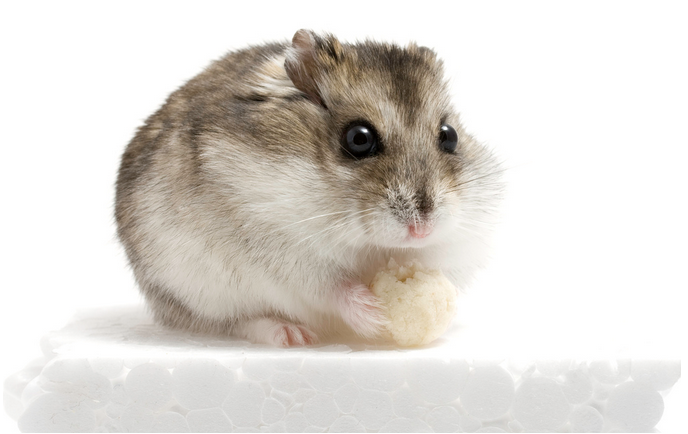
\includegraphics[height=3cm]{cricetulus2.png}
            \item Find some interesting information about it in the database.
            \item Tweet to me a piece of information with the hashtag \url{\#cricetulus}.
            \item Get a coffe mug for an interesting tweet!
        \end{itemize}
    \end{frame}
    
\end{document}